\section{Performance}

\begin{frame}[fragile]
	\frametitle{TODO}
	Benchmarks run with
\begin{lstlisting}
npart=1000000
tevol_dt=0.00100000000
theta=0.400000
max_iter=20
\end{lstlisting}
	Compiled with \lstinline|O3|.
\end{frame}

\begin{frame}
	\frametitle{Strong Scaling}
	\begin{figure}
		\centering
		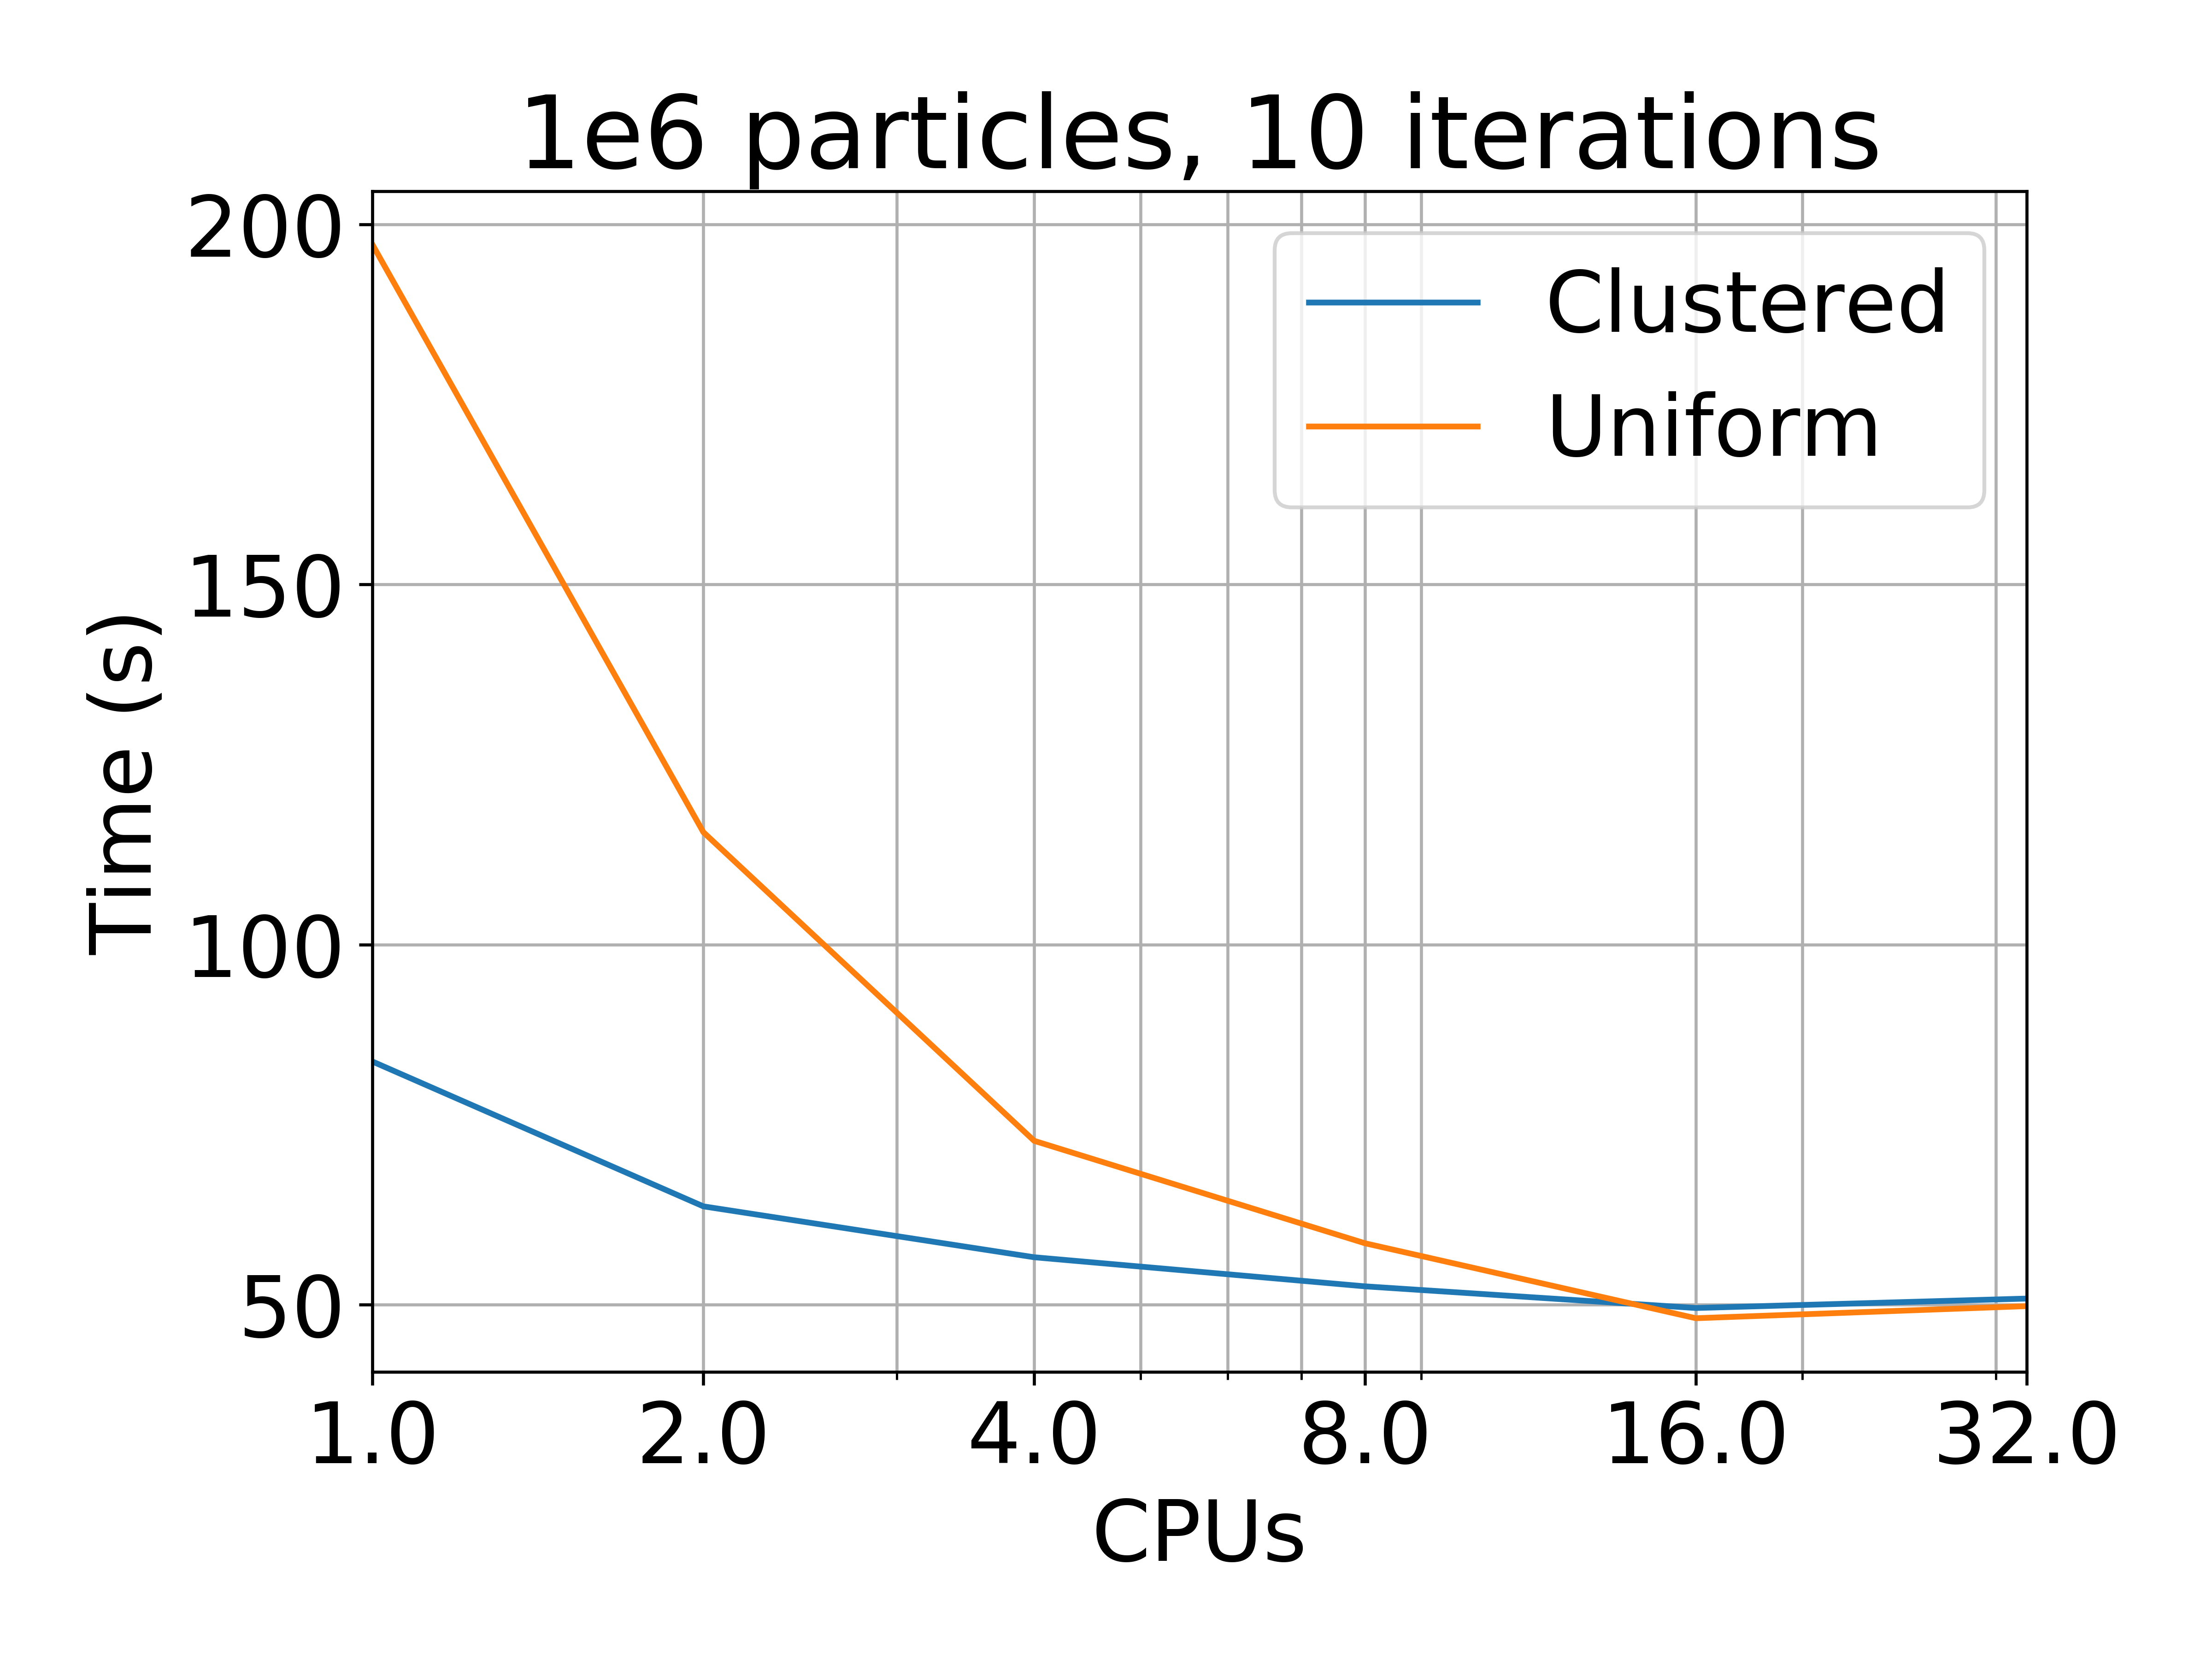
\includegraphics[width=0.49\textwidth]{inclfigs/strong_time.png}
		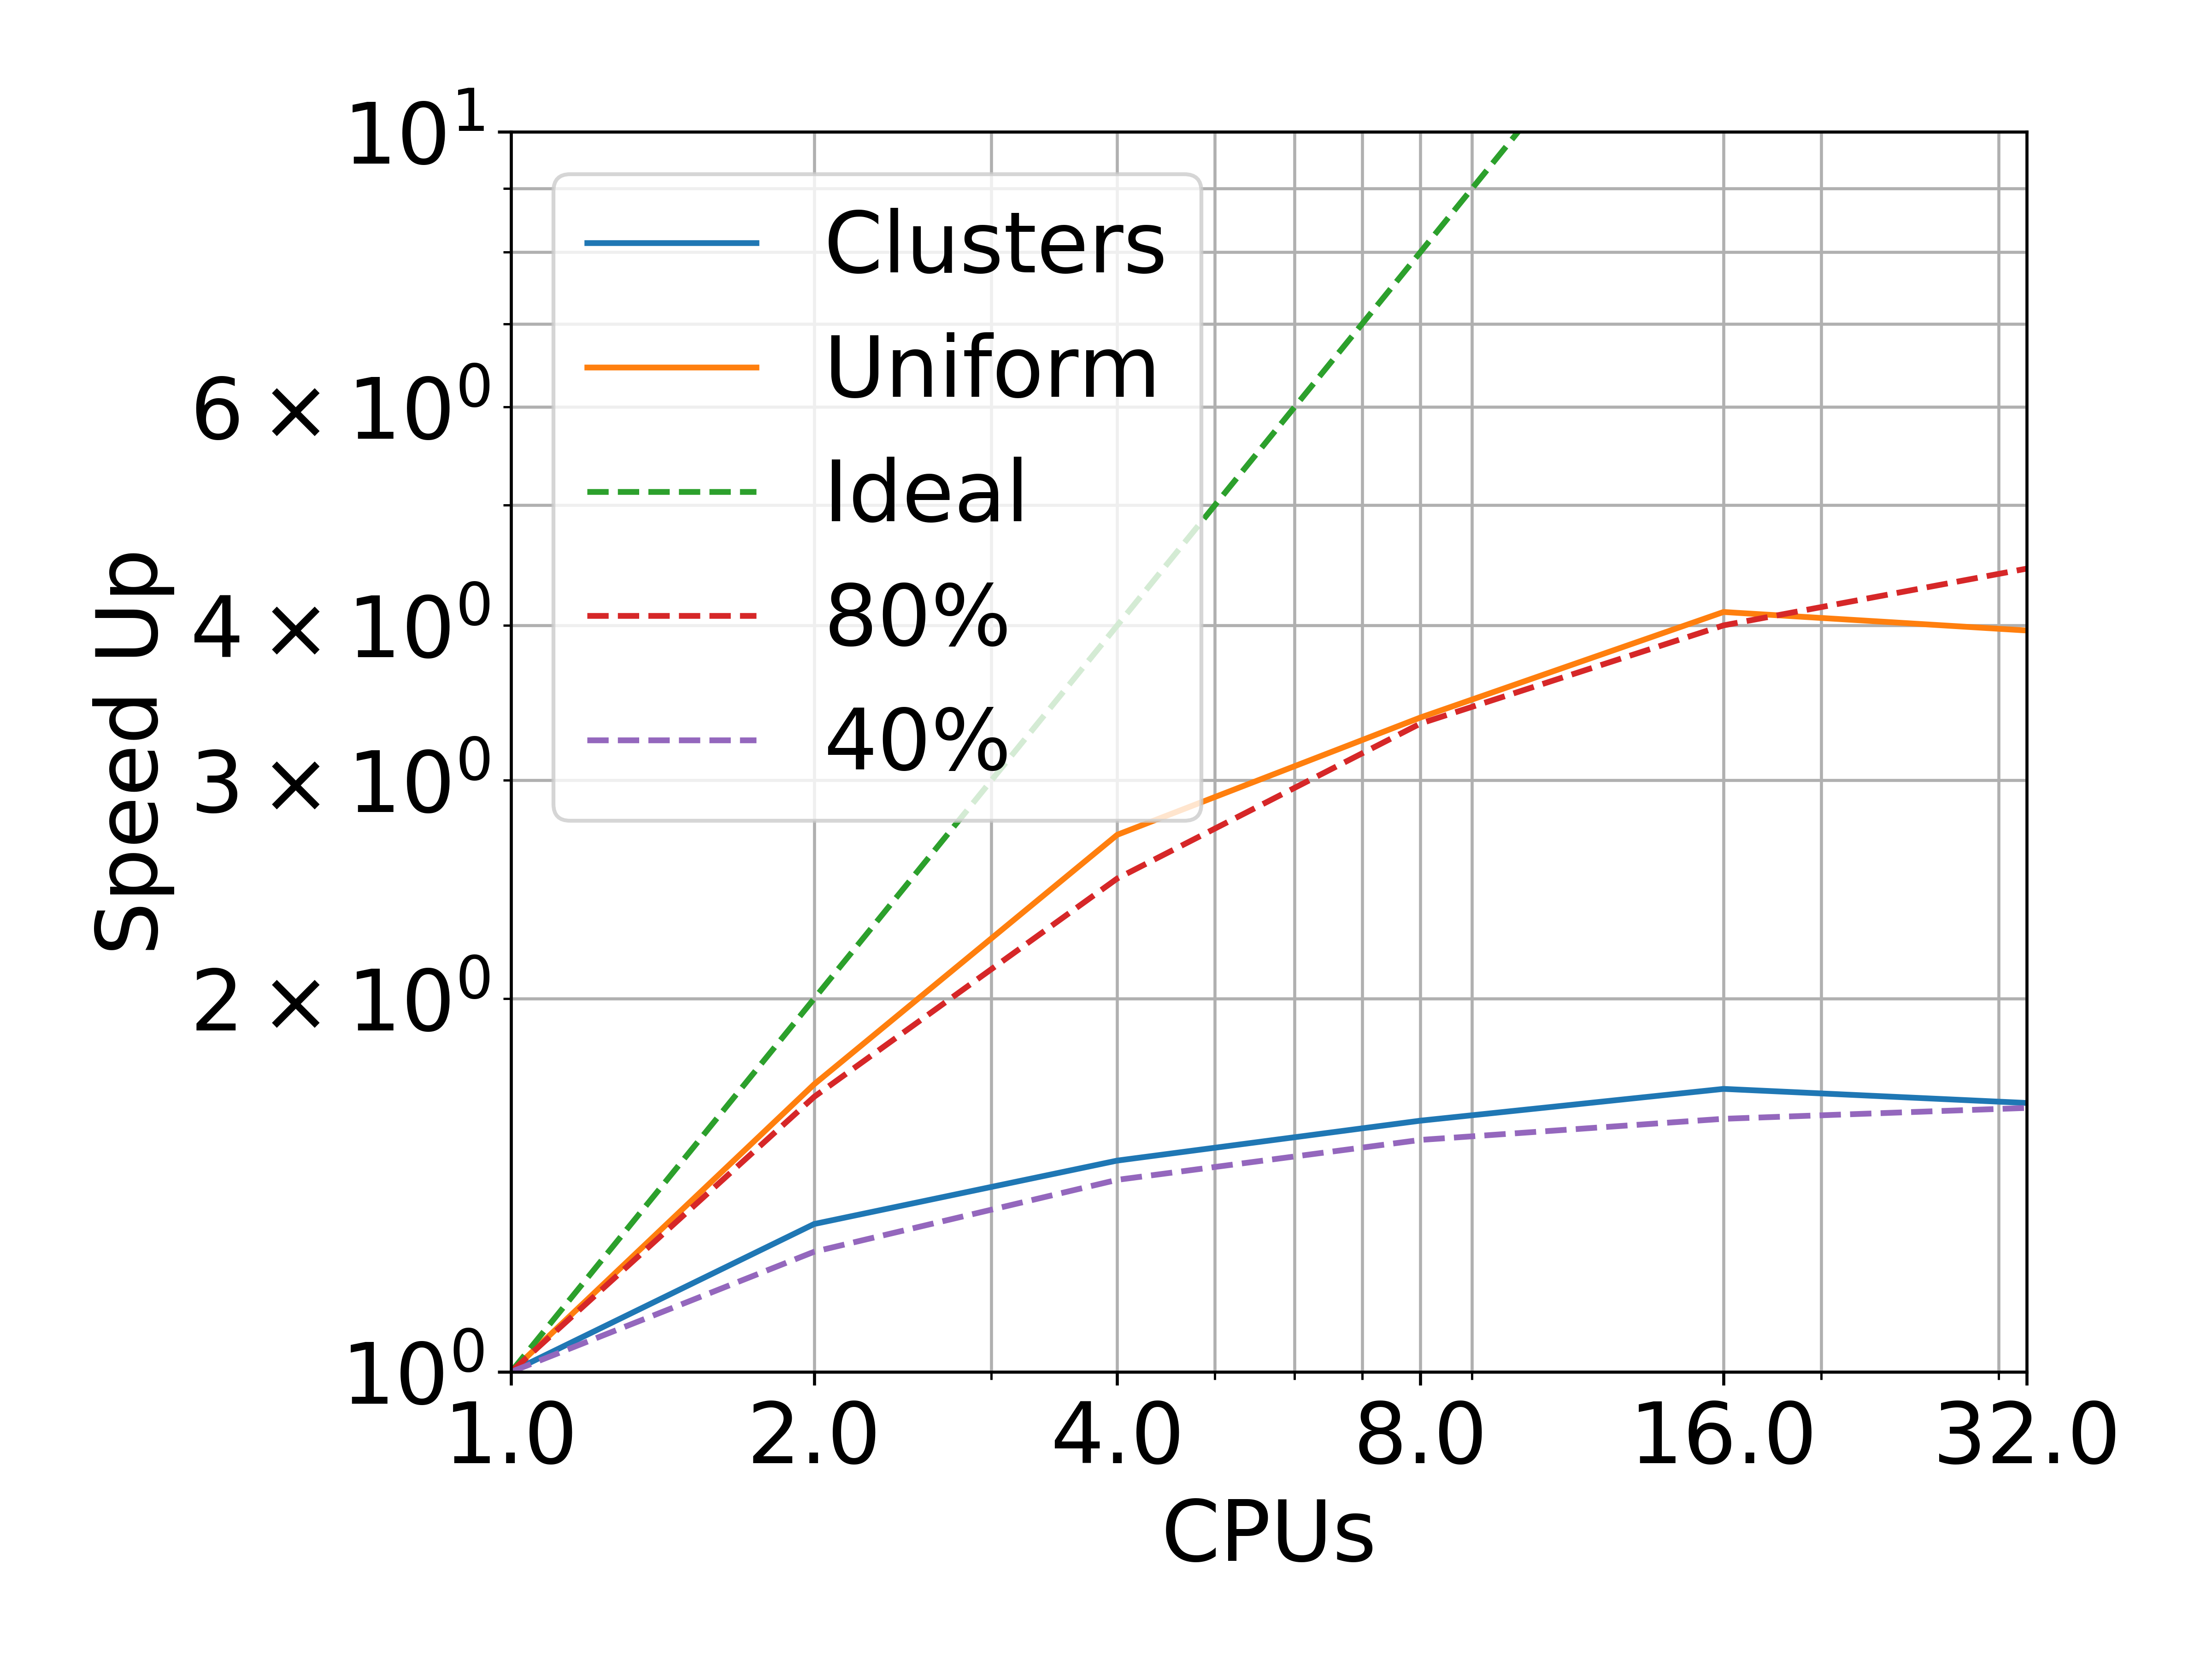
\includegraphics[width=0.49\textwidth]{inclfigs/strong_speedup.png}
	\end{figure}
\end{frame}

\begin{frame}
	\frametitle{Weak Scaling}
	\begin{figure}
		\centering
		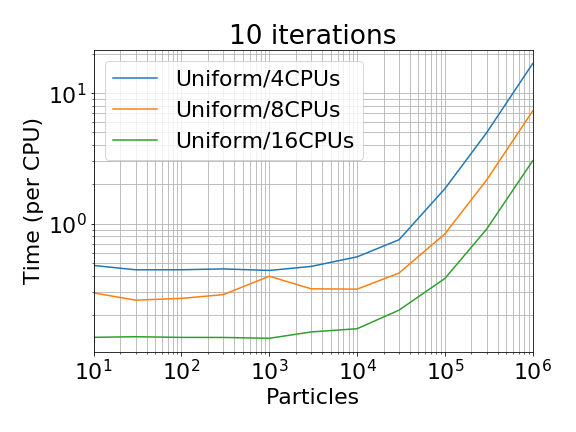
\includegraphics[width=0.49\textwidth]{inclfigs/weak_time.png}
		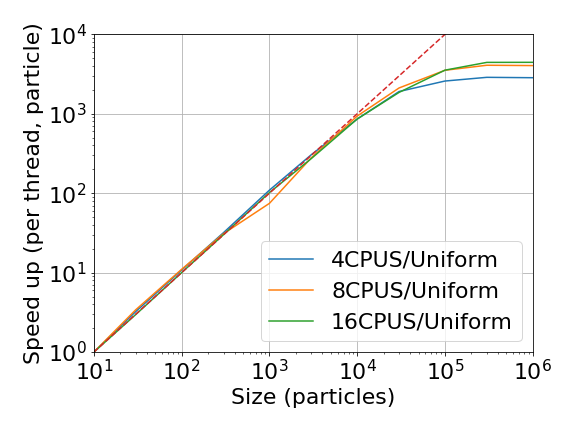
\includegraphics[width=0.49\textwidth]{inclfigs/weak_speedup.png}
	\end{figure}
\end{frame}

\begin{frame}
	\frametitle{Hotspots}
	\begin{figure}
		\centering
		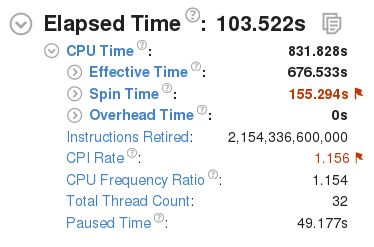
\includegraphics[width=0.49\textwidth]{inclfigs/par-spintime.png}
		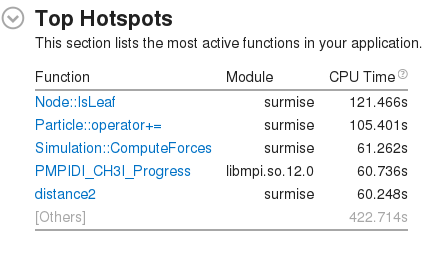
\includegraphics[width=0.49\textwidth]{inclfigs/par-hotspots.png}
	\end{figure}
\end{frame}

\begin{frame}
\frametitle{Bottom-Up}
	\begin{figure}
		\centering
		\only<1>{\makebox[\textwidth]{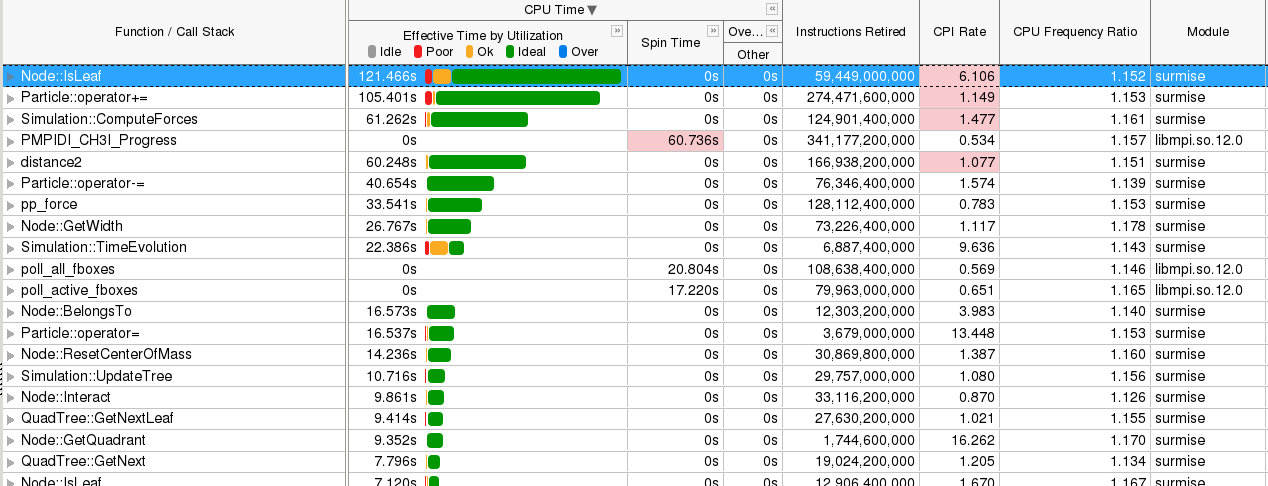
\includegraphics[width=\paperwidth]{inclfigs/par-bottomup.png}}}
		\only<2>{\makebox[\textwidth]{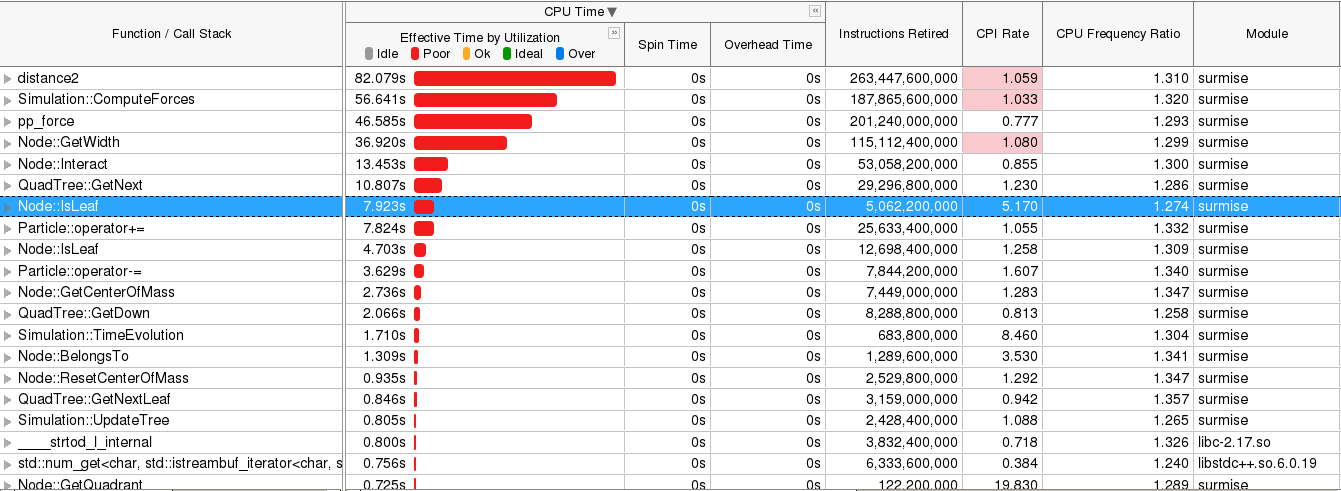
\includegraphics[width=\paperwidth]{inclfigs/seq-bottomup.png}}}
	\end{figure}
\end{frame}

\begin{frame}
\frametitle{CPU Time}
	\begin{figure}
		\centering
		\makebox[\textwidth]{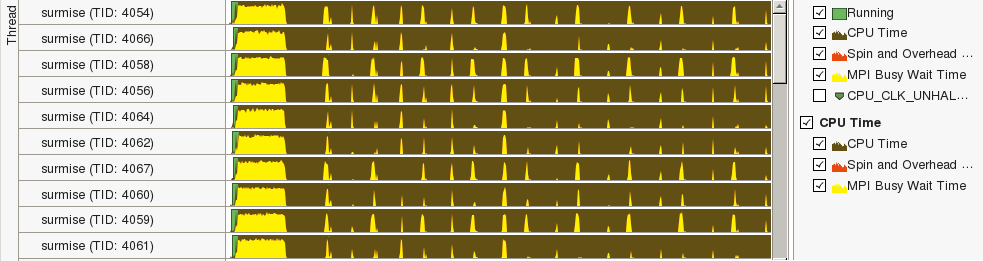
\includegraphics[width=\paperwidth]{inclfigs/par-heatmap.png}}
	\end{figure}
\end{frame}